\documentclass{article}

\setlength{\parindent}{0pt}
\usepackage[round]{natbib}

\usepackage{graphicx}
\graphicspath{ {./images/} }

\title{Simulation of Tree Growth}
\date{2020-12-01}
\author{Eric Ekström}
	
\begin{document}
	
	\pagenumbering{gobble}
	\maketitle
	\newpage
  	
  	\section*{Abstract}
  	
  	\newpage
  	\tableofcontents
  	\newpage
  	\pagenumbering{arabic}

  	\section{Introduction}
  		 
  	\section{Background}
  		
  		
  		\subsection{Tree Structure and Terminology}
  			This section covers the terminology used when describing trees. The choice of language is based on the description of trees by \citep{barthelemy2007plant}. \\
  			
  			A tree consists of a number of nodes. Each node supports nodes further out in the tree.
  			
  			\begin{itemize}
  				\item A \textit{node} is the main component of the tree. It supports at least a bud, another node or a leaf. A node combined with an internode is called a \textit{metamer}. \citep{barthelemy2007plant}
  				\item An \textit{internode} is the section of stem between two nodes.
  				\item The \textit{lateral branch} is a supported node that is connected at an angle  to the supporting node.
  				\item The \textit{main branch} is a supported node that has the same angle as the supporting node.
  				\item \textit{Buds} are potential points for expansion of new nodes. A lateral bud is located at the node that already has a main branch. An apical bud is located at a node that has no branches to support.
  				
  			\end{itemize}
  			
  			For this project, a tree grows by shooting a number of new metamers from a bud. This is called rhythmic growth and is the more commonly observed method of growth in nature. \citep{barthelemy2007plant} The fate of a bud and the number of new metamers depends on a number of factors. For this project, only a simulated light resource was considered.\\
  			
  			A node is given an order based on the number of node below it. A node without a supporting node has order 1.
  		\subsection{Volumetric Light Scattering}
  			Volumetric light scattering (also called "godrays" or "crepuscular rays") is a light phenomenon that occurs when the mixture of gas and molecules in the air is just right. This causes light to be rayleigh-scattered and creates visual sun beams through the air. (See Figure \ref{fig:godrayexample}.)
  			
  			\begin{figure}[h!]
  				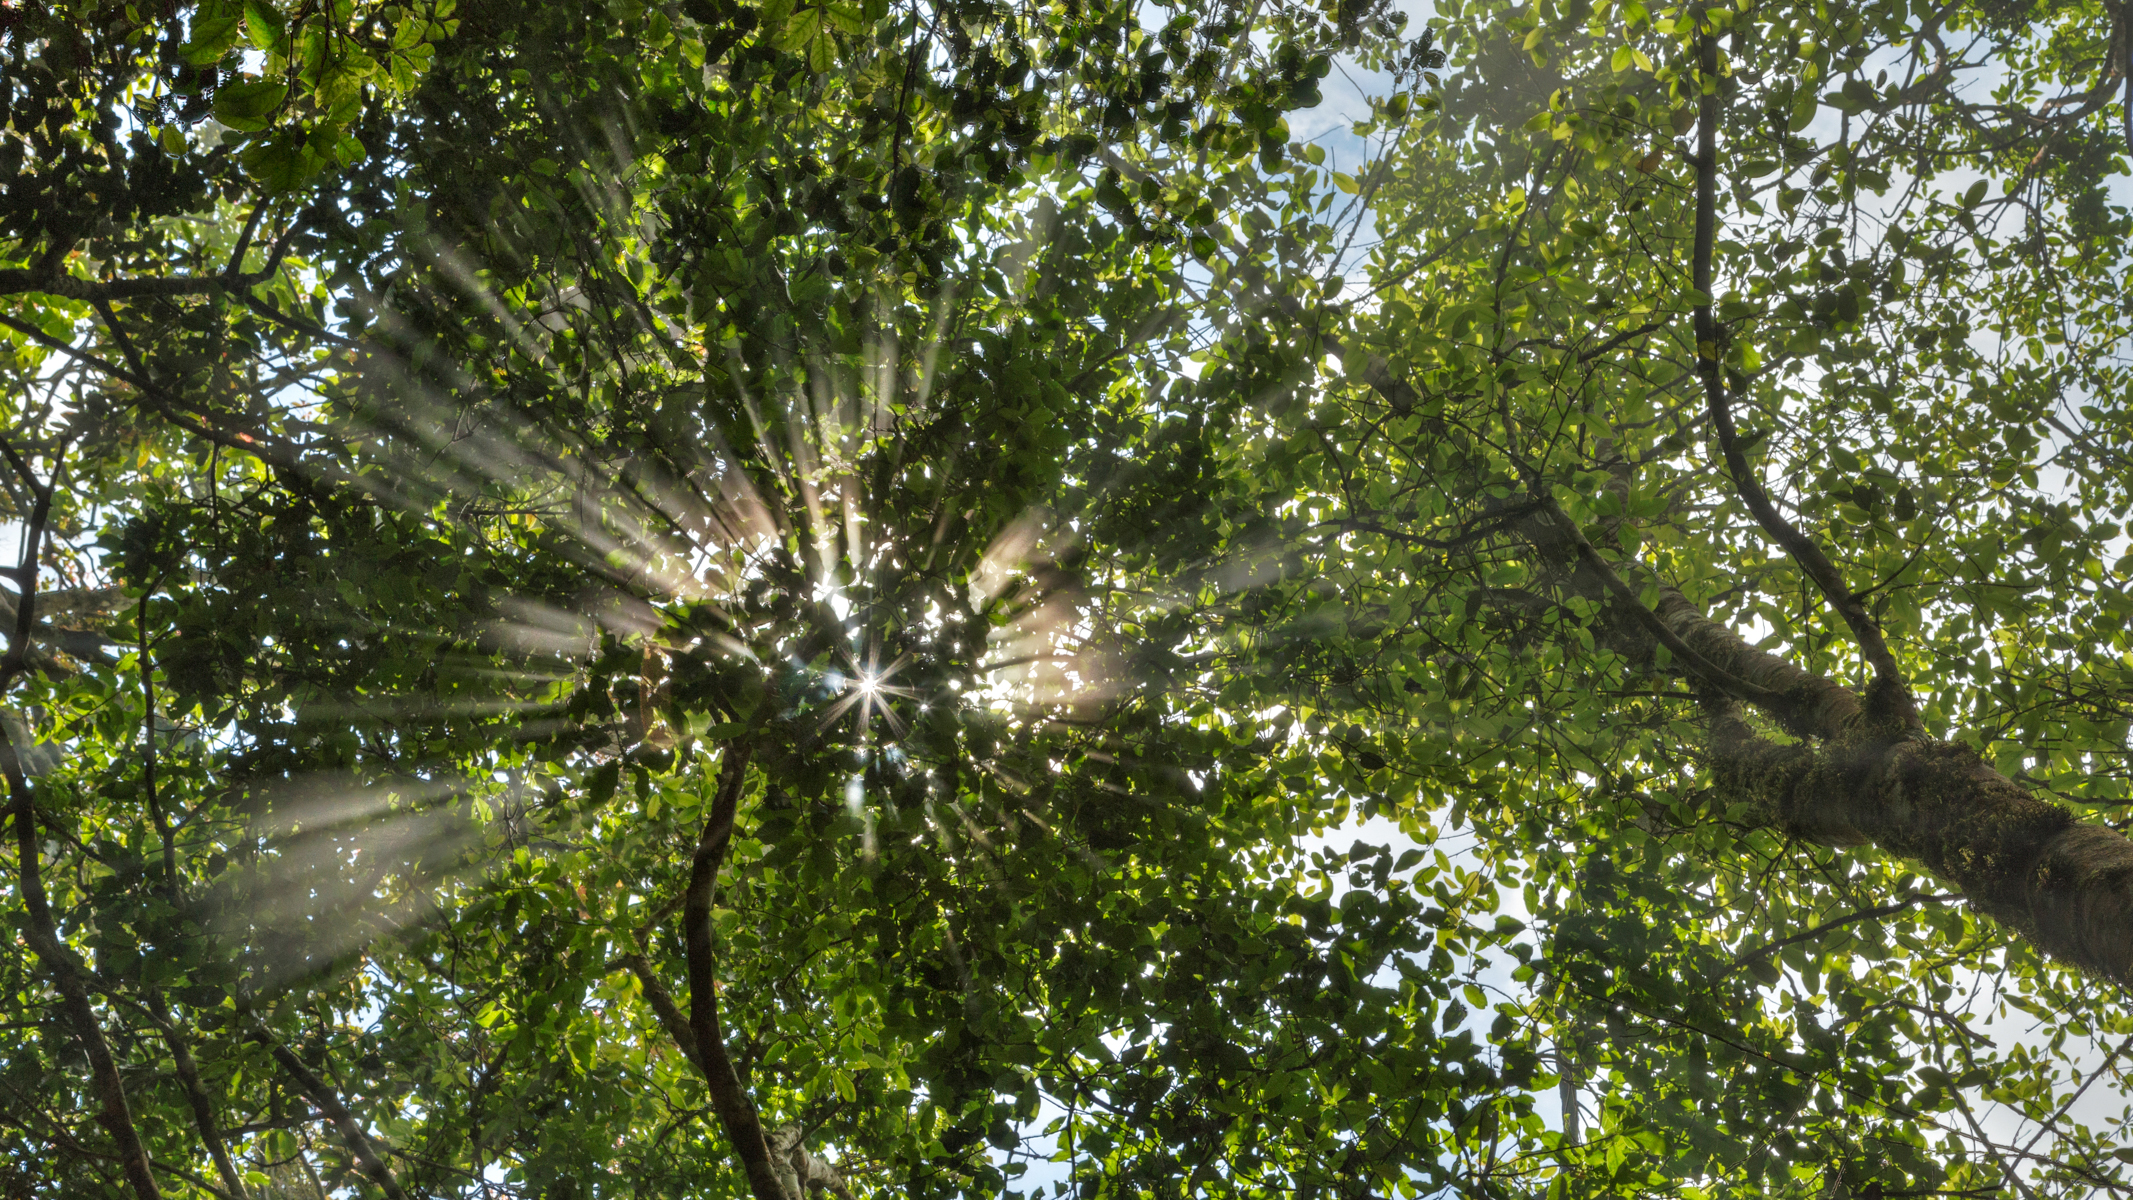
\includegraphics[scale=0.7]{godrays}
  				\caption{An example of volumetric light scattering. (Sunshine Kodai Kanal, Manoj K Racherla, 2013)}
  				\label{fig:godrayexample}
  			\end{figure}
  			
  		
  			
  	\section{Method}
  		\subsection{Tree Generation}
  			
  		\subsection{Volumetric Light Scattering}
  		
  		\subsection{Shadow Mapping}
  			
  	\section{Result}
  		
  	\section{Discussion}
  		
  	\subsection{Improvements}

	\newpage
	\bibliographystyle{plainnat}
	\bibliography{ref}{}
  		
\end{document}
